% Chapter 3

\chapter{Grundlagen} % Main chapter title

\label{Chapter3} % For referencing the chapter elsewhere, use \ref{Chapter1}

%----------------------------------------------------------------------------------------

\begin{itquote}
``To deal with hyper-planes in a 14-dimensional space, visualize a 3-D space and say `fourteen' to yourself
very loudly. Everybody does it.''
\flushright
\textsc{Geoffery Hinton}
\end{itquote}

\section{Neurale Netzwerke}

Wie der Name bereits erahnen lässt, fußt die Idee von neuralen Netzwerken auf einer mathematischen Modellierung
des menschlichen Gehirns (siehe Abbildung \ref{fig:perceptron} und (\cite{rosenblatt1958perceptron})). Die Grundbausteine bilden dabei einzelne Neuronen, die dabei auf folgende Art und Weise
modelliert werden (dieser Teil ist dabei auch als \emph{Perceptron}-Algorithmus bekannt):

\begin{figure}[h]
  \centering
  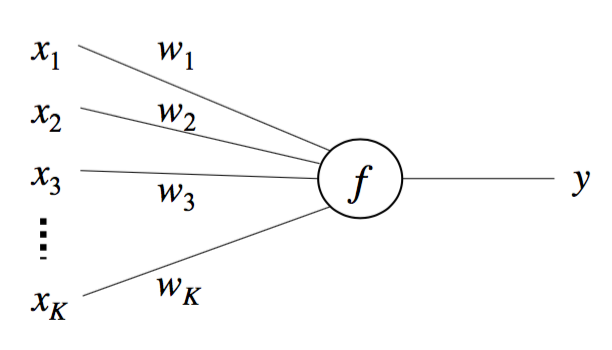
\includegraphics[width=0.65\textwidth]{../img/neuron.png}
  \caption[Mathematische Modellierung eines Neurons]{Mathematische Modellierung eines Neurons, auch bekannt als
  \emph{Perceptron}-Algorithmus von (\cite{rosenblatt1958perceptron}). $x$ bezeichnet In-, $y$ den Output des Neurons, $w$ bilden die Gewichte und $f$ die
  Aktivierungsfunktion. Abbildung aus (\cite{rong2014word2vec}).\label{fig:perceptron}}
\end{figure}

Der Analogie der menschlichen Nervenzelle folgend erhält das Neuron mehrere Inputs in Form eines Vektors $x$ mit $K$
Dimensionen. Der Output erhält die Bezeichnung $y$. Um den Output zu bestimmen enthält die Zelle eine Aktivierungsfunktion
$f$ (um zu bestimmen, wann das Neuron ``feuert''):
\begin{equation}
  y = f(u)
\end{equation}

$u$ bezeichnet dabei einen Skalar, dem man durch das Summieren der mit $w$ gewichteten Inputs erhält:
\begin{equation}
  u = \sum_{i=0}^{K} w_i x_i = w^T x
\end{equation}

Für die Aktivierungsfunktion $f$ bieten sich mehrere Optionen. Ursprünglich wurde die \emph{Heaviside step function}
oder \emph{Rectifier (ReLU)} (siehe bspw. (\cite{abramowitz1964handbook})) gewählt:
\begin{equation}
    f(u) = \begin{cases} 1 & \quad \text{if}\ u > 0 \\ 0 & \quad \text{otherwise} \\ \end{cases} \text{bzw.} \\
\end{equation}
\begin{equation}
  f(u) = max(0,u) = \begin{cases} 0 & \quad \text{if}\ u < 0 \\ u & \quad \text{otherwise} \end{cases}
\end{equation}

Andere Funktionen sind z.B. \emph{sigmoid} ($\sigma(u) \in [0,1]$)
und \emph{tanh} ($tanh(u) \in [-1, 1]$), im Gegenteil zu den beiden zuvor sind diese durch ihre s-förmige Form
kontinuierlich und dadurch ableitbar:

\begin{equation}
  \sigma(u) = \frac{1}{1 + e^{-u}}
\end{equation}
\begin{equation}
  tanh(u) = \frac{e^{2u}-1}{e^{2u}+1}
\end{equation}

In der jüngeren Vergangenheit fand jedoch wieder eine Rückkehr zu den alten Funktionen statt, siehe z.B. (\cite{maas2013rectifier}).

Um aus einzelnen Neuronen nun ein neurales Netzwerk zu kreieren, werden mehrere Schichten erstellt (i.d.R. eine Eingabe-
(\emph{input layer}), eine Ausgabe- (\emph{output layer}) und min. eine ``versteckte'' Schicht (\emph{hidden layer}).
Die Schichten bestehen dann aus mehreren parallelen Zellen, wobei jede Zelle mit jeder anderen Zelle der vorhergehenden und
folgenden Schicht vernetzt ist (siehe Abbildung \ref{fig:neuralnet})\footnote{Dabei gibt es aber auch Netzwerke, bei denen
absichtlich Verbindungen ignoriert werden oder Nervenzellen mit Zellen aus einer anderen Schicht als der nächstvorderen
verknüpft sind.}.

\begin{figure}[h]
  \centering
  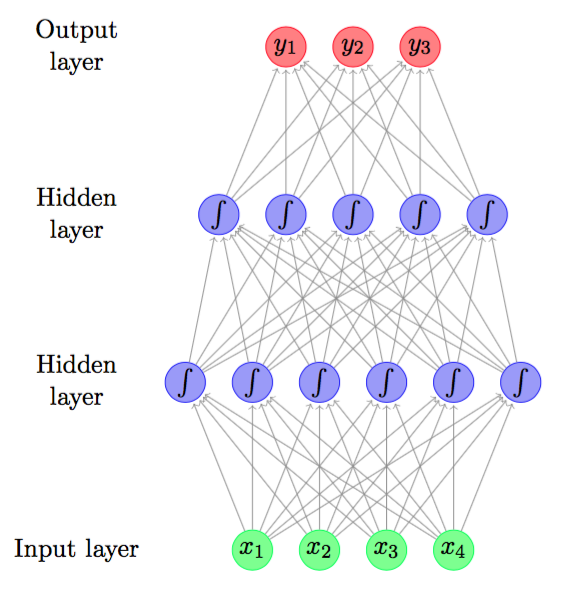
\includegraphics[width=0.5\textwidth]{../img/neuralnet.png}
  \caption[Darstellung eine neuralen Netzwerks]{Darstellung eines neuralen Netzwerks mit vier Schichten, davon jeweils eine
  für In- und Output, sowie zwei ``versteckte'' Schichten (\emph{hidden layer}). Bild aus (\cite{Goldberg15c}).\label{fig:neuralnet}}
\end{figure}

Die einzelnen Gewichtsvektoren $w$ aller Neuronen einer Schicht werden dann i.d.R. zu einer Gewichtsmatrix $W$ zusammengefasst,
wobei jede Zeile einem Gewichtsvektor entspricht. Zum Training dieser Strukturen wird der sog. \emph{Backpropagation}-Algorithmus verwendet, der mithilfe einer vorher definierten Verlustfunktion (die anzeigt, inwiefern das durch das Netzwerk
erzeugt Ergebnis von dem erwünschtne Ergebnis abweicht) einen Fehler errechnet. Dieser wird rekursiv durch alle
Schichten des Netzwerks zurückgegeben und simultan die Werte innerhalb der Gewichtsmatrix anpasst.

\section{Wortvektoren}\label{sec:wordvec}

Frühere Experimente mit Wortvektoren arbeiteten meist mit sog. ``One-Hot''-Vektoren, bei denen jede Dimension i.d.R.
einem betimmten Wort zugeordnet wurde. Nehmen wir beispielsweise das Minikorpus ``Der Hund beißt den Mann'' an.
Das Vokabular besteht dann aus $\textsc{V} = \{beißt,\ Der,\ den,\ Hund,\ Mann\}$ (in alphabetischer Reihenfolge).
Um jedes dieser Wörter als einen der oben genannten Vektoren zu repräsentieren, können wir Vektoren der Länge $V$\footnote{
$V$ steht eigentlich für $\|\textsc{V}\|$, wird der Übersicht halber aber im Folgenden stellvertrentend dafür verwendet.}
benutzen. Um nun zum Beispiel einen Vektor für \emph{Hund} zu generieren, setzen wir den Wert der Stelle des Vektors (=
\emph{Feature}) auf $1$, der dem Index von Hund in $\textsc{V}$ entspricht,
also $\vec{v}(Hund)=(0, 0, 0, 1, 0)$.\\
Diese Art von Wortvektor wird gemeinhin als ``sparse'', also spärlich bezeichnet, da sie relativ wenig Information enthält.
\emph{Wortkontextvektoren}\footnote{Im Englischen zur Abgrenzung \emph{word embeddings}
genannt.}, die mithilfe von Neuralen Netzwerken trainiert werden, beinhalten mehr (semantische) Informationen über das dazugehörige Wort, zudem lassen sich einzelne Features
nicht mehr auf eindeutig auf bestimmte Worte zurückführen\footnote{Die semantische Information ist \emph{implizit} in der
Vektorrepräsentation kodiert.}. Ein populäres Werkzeug zu diesem Zweck ist \verb|word2vec| von (\cite{mikolov2013efficient}).\\

Das Training dieser neuen Wortkontextvektoren läuft folgendermaßen ab:
Als Input fungieren die erwähnten ``One-Hot''-Vektoren, welche genau so viele Dimensionen wie Worte im Vokabular besitzen
($\vec{v} \in \mathbb{R}^V$).
Die Modelle bestehen aus drei Schichten, namentlich \emph{Input}, \emph{Hidden} und \emph{Output}.
Input und Output besitzen die Dimensionalität von $V$, Hidden die von $N$, was die gewünschte Anzahl der Dimensionen der
Wortkontextvektoren entspricht.\\

\begin{figure}[h]
  \centering
  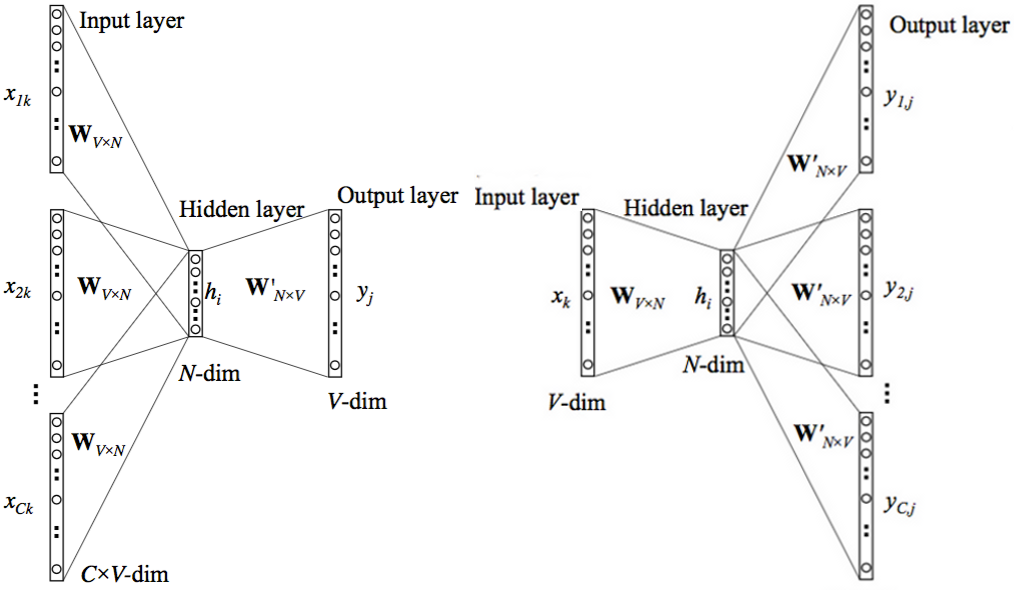
\includegraphics[width=1.1\textwidth]{../img/cbowskip.png}
  \caption[Gegenüberstellung von Skip-Gram und CBOW]{Gegenüberstellung der beiden Trainingsmethoden CBOW (links)
  und Skip-Gram (rechts). CBOW versucht die Wahrscheinlichkeit eines Wortes gegeben seines Kontexts zu trainieren,
  Skip-Gram die Wahrscheinlichkeit eines Kontextes gegeben eines Wortes. Modifizierte Abbildung nach
  (\cite{rong2014word2vec}).\label{fig:cbowskip}}
\end{figure}

Zwischen Input und Hidden liegt die Gewichtsmatrix $W$ und zwischen Hidden und Output die Matrix $W'$.
CBOW versucht, die Wahrscheinlichkeit eines Wortes gegeben eines Kontextes
der Größe $C$\footnote{Kontext bezieht sich in diesem Fall auf die Summe der rechts und links vom Eingabewort stehenden
Wörter, siehe Abbildung \ref{fig:cbowskip}.} zu maximieren. Unsere Verlustfunktion, deren Wert es dabei zu minimieren gilt,
besteht darin in der negativen logarithmischen Wahrscheinlichkeit eines Wortes gegeben seines Kontextes:

\begin{equation}
  E = - log\ p(w_O | w_{I,1}, \ldots, w_{I,C})
\end{equation}

Beim Skip-gram-Modell verhält sich das Ganze genau umgekehrt, es wird versucht, den Kontext gegeben eines Eingabewortes
vorherzusagen:

\begin{equation}
  E = - log\ p(w_{I,1}, \ldots, w_O)
\end{equation}

In beiden Fällen wird daraufhin überprüft, ob die Vorhersage mit den tatsächlichen Daten übereinstimmt und die Abweichung
errechnet, mit der dann die Parameter der Gewichtsmatrizen $W$ und $W'$ rekursiv angepasst werden, um zukünftige Prognosen
zu verbessen, wofür der \emph{Backpropagation}-Algorithmus verwendet wird. Die Wortkontextvektoren, die dann nach dem Durcharbeiten aller Trainingsdaten resultieren, sind dann die Zeilen von
$W'$, wobei die \emph{i}-te Zeile der Matrix dem Wortvektor des Wortes mit dem Index \emph{i} im Vokabular entspricht.\\

Eigentlich erfordert das Training eine aufwendige Berechnung über alle Wörter des Vokabulars, was der Skalierbarkeit dieses
Verfahrens entgegensteht. Der computationelle Aufwand kann allerdings durch Techniken wie \emph{Hierarchisches Softmax}, bei dem
der Aufwand durch einen binären Baum von $O(V)$ auf $O(log\ V)$ verkleinert wird sowie
\emph{Negativem Sampling} reduziert werden (\cite{rong2014word2vec}; \cite{goldberg2014word2vec}).
Bei letzterem werden ``schlechte'' (also Negativ-)Beispiele zum Training hinzugezogen, woher sich auch der Name des Verfahrens ableitet.\\

%\section{Wortvektoren aus Dependenzen}
%
%Dependenzgrammatiken untersuchen die Abhängigkeiten zwischen Wörtern eines Satzes und fügen diese in eine Dependenzstruktur ein.
%Anders als in der Phrasenstrukturgrammatik entsteht dabei kein Syntaxbaum mit Knoten. Worte stehen in Abhängigkeitsverhältnissen,
%wobei das das die Dependenz verursachende Wort alt \emph{Regens}, das davon abhängige als \emph{Dependenz} bezeichnet wird.\\
%(\citeauthor{levy2014dependency}) machen sich dies zunutze, um den Kontext beim Training von Wortvektoren neu zu definieren:
%Er besteht nun nicht mehr als den umgebenden Wörtern im Satz, sondern aus den Depenzen: Für ein Word $w$ mit den Modifizierern
%$m_1, \ldots m_k$ und den Kopf $h$ besteht der Kontext nun aus $(m_1, lbl_1), \ldots (m_k, lbl_k), (h, lbl_h^{-1})$, wobei
%$lbl$ stellvertretend für eine Dependenzrelation steht, ein $-1$ im Exponenten zeigt das Inverse einer solchen Relation an.
%Ein Beispiel dafür ist in Abb. X zu sehen.\\

%\begin{figure}[h]
%    \centering
%    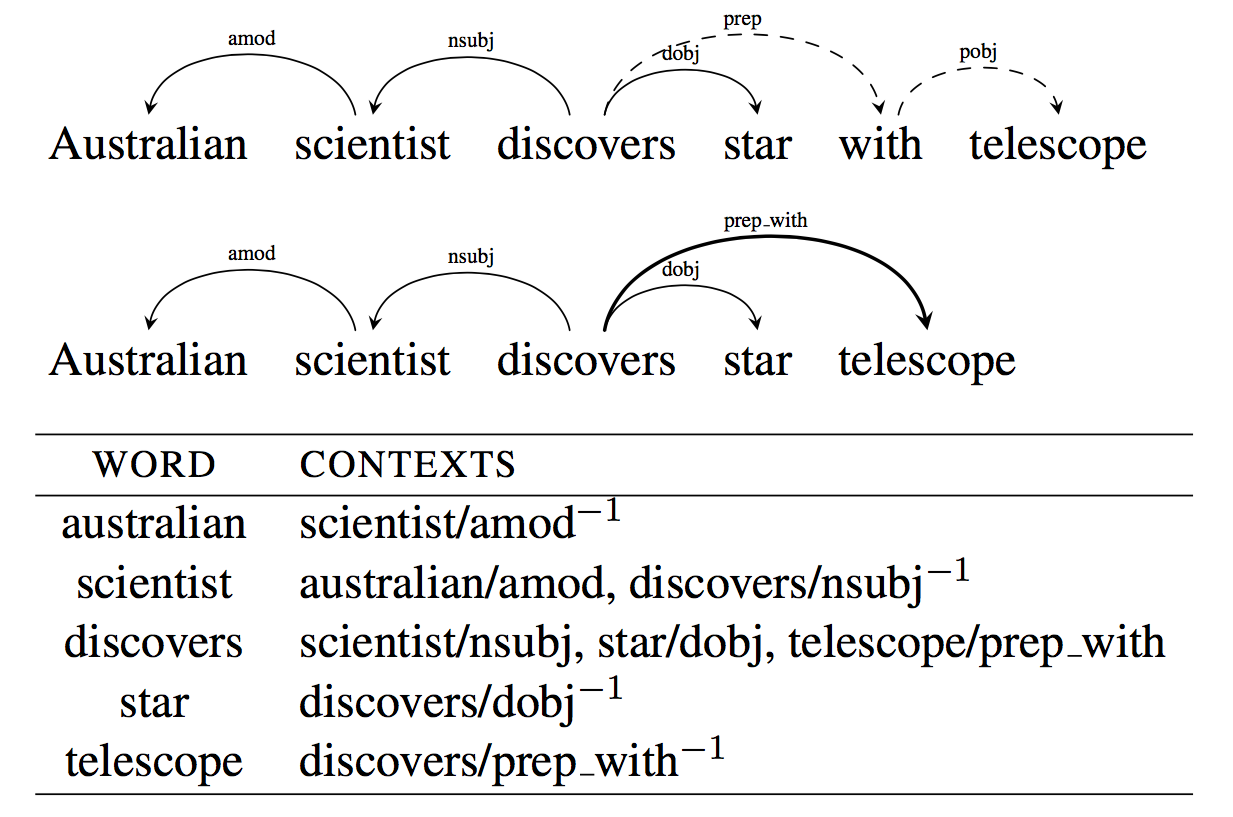
\includegraphics[scale=0.2]{../img/depend_ex.png}
%    \caption[Erstellung von Dependenzkontexten beim Wortvektortraining]{Beispiel der Erstellung von Wortkontexten aus Dependenzen.
%    Dependenzen mit Präposition werden zu einer Abhängigkeit zusammengefasst. \textbf{Oben}: Dependenzstruktur.
%    \textbf{Unten}: Extrahierte Kontexte.}
%\end{figure}

\section{Clustering}

\emph{Clustering} bezeichnet eine Art von unüberwachten maschinellen Lernen,
die versucht, Elemente, die nach vorher definierten Maßgaben als ähnlich erachtet
werden sollen, zu gruppieren.\\
Die Literatur zu diesem Thema bietet dabei eine Fülle von Algorithmen mit verschiedenen
Grundannahmen, aus denen es zu wählen gilt. Für die Aufgaben in dieser Arbeit wurde
der DBSCAN-Algorithmus (\textbf{D}ensity-\textbf{B}ased \textbf{S}patial \textbf{C}lustering of
\textbf{A}pplications with \textbf{N}oise) von (\cite{ester1996density}) gewählt, da er folgende Kriterien erfüllt:
\begin{itemize}
  \item DBSCAN erlaubt es, dass nicht alle Datenpunkte nach der
  Terminierung des Algorithmus einem Cluster zugeordnet sein müssen (\emph{Outlier detection})
  \item Die Anzahl der Cluster muss bei Beginn des Algorithmus nicht festgelegt werden.
  \item Cluster werden nicht nach der räumlichen Distanz zwischen den Punkten gebildet, sondern nach deren
  Dichte im Raum. Dies lässt auch nicht-sphärische Clusterformen zu\footnote{Vgl. dazu z.B. \url{http://scikit-learn.org/stable/modules/clustering.html}.}.
\end{itemize}

Zur Erklärung von DBSCAN müssen zuerst einige Definitionen erstellt werden (siehe Abbildung \ref{fig:dbscan} zur visuellen
Darstellung):
\begin{itemize}
  \item Ein Punkt $p$ in den Daten wird dann als
  Kernpunkt (\emph{core point}) bezeichnet, sofern mindesten $minPts$ Punkte innerhalb einem Radius $\epsilon$ vorhanden sind.\\
  Diese Punkte sind von $p$ \emph{direkt erreichbar}.
  \item Ein Punkt $q$ ist von $p$ erreichbar, sofern es einen Pfad $p_1, \ldots, p_n$ mit $p_1 = p$ und $p_n = q$ gibt, wobei
  jeder Punkt $p_{i+1}$ von einem Punkt $p_i$ direkt erreichbar ist.
  \item Alle Punkte, die nicht von einem anderen Punkt aus direkt erreichbar sind, sind Ausreißer (\emph{Outlier}).
  \item Zwei Punkte $p$ und $q$ sind \emph{direkt verbunden}, sofern es einen Punkt $o$ gibt,
  von dem aus beide Punkte direkt erreichbar sind.
  \item Cluster bestehen aus Punkten, die alle miteinander direkt verbunden sind.
\end{itemize}

\begin{figure}[h]
  \centering
  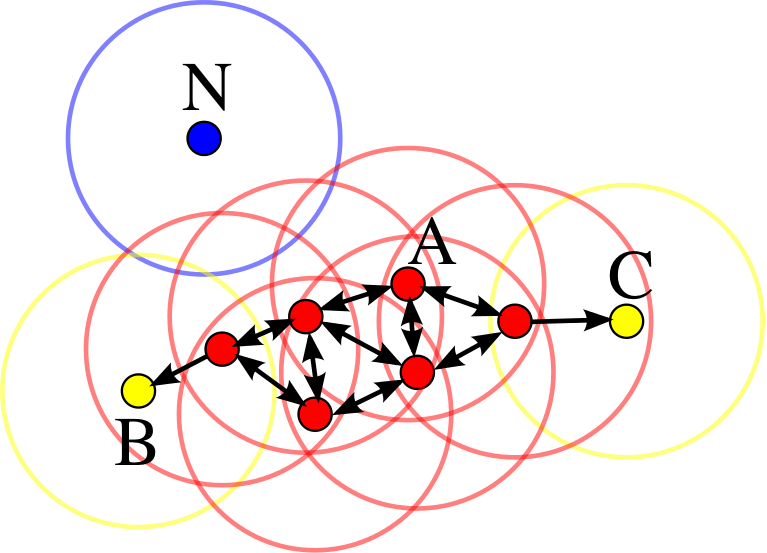
\includegraphics[width=0.6\textwidth]{../img/DBSCAN-Illustration.png}
  \caption[Darstellung der Funktionsweise von DBSCAN]{Darstellung der Funktionsweise von DBSCAN. Punkt A ist ein Kernpunkt, die
  Punkte B und C sind von A aus erreichbar. Punkt N ist nicht erreichbar und damit ein Ausreißer.\label{fig:dbscan}\footnotemark}
\end{figure}
\footnotetext{Abbildung von
Chire - Eigenes Werk, CC BY-SA 3.0, \url{https://commons.wikimedia.org/w/index.php?curid=17045963} (zuletzt abgerufen am
25.04.16).}

Der Algorithmus ist von linearer Komplexität, sofern ihm eine geeignete Indexierung der Daten zugrunde gelegt wird, ansonsten
verhält sich die Komplexität quadratische zur Anzahl der Datenpunkte\footnote{Bei der
\verb|scikit-learn|-Implementation wird beispielsweise ein Nearest-Neighbour-Graph verwendet:
\url{http://scikit-learn.org/stable/modules/generated/sklearn.cluster.dbscan.html} (zuletzt abgerufen am 25.04.16)}.\\

Versuche, den Algorithmus zu parallelisieren und somit eine bessere Skalierbarkeit zu ermöglichen wurden beispielsweise von
(\cite{arlia2001experiments}) unternommen. Solche Vorgehen sind wichtig, um die Skalierbarkeit des Algorithmus auf große
Datenmengen wie beispielsweise in Kapitel \ref{Chapter7} zu sichern.
